\documentclass{article}
\usepackage[utf8]{inputenc}
\usepackage{amsmath}
\usepackage{amsfonts}
\usepackage{graphicx}
\usepackage{multicol}
\usepackage{float}
\usepackage{cite}
\usepackage{url}
\usepackage{listings}
\usepackage{pythonhighlight}

\begin{document}
	\begin{titlepage}
		\begin{center}
			{\huge\textbf{Instituto Politécnico Nacional}}\\
			\vspace{7mm}
			{\huge\textbf{Escuela Superior de Cómputo}}\\			
			\begin{figure}[h]
				\centering
				
\includegraphics[height = 6cm]{logoEscom.png}
			\end{figure}	
			\vspace{1cm}
			{\huge\textbf{Programa 5: Expresión Regular}}
			\par\vspace{2cm}
			\large\textbf{Autor: Colín Ramiro Joel}
			\par\vspace{1cm}
			{\large\textbf{Materia: Teoría de la Computación}}
			\par\vspace{1cm}
			{\large\textbf{Grupo: 4CM2}}
			\par\vspace{1cm}
			{\large\textbf{Profesor: Juarez Martínez Genaro}}
			\par\vspace{1cm}
			{\large\textbf{Fecha de entrega: {\huge{29 de Diciembre 2021}}}}
			\par\vspace{3cm}
		\end{center}
	\end{titlepage}

	\section*{Introducción}
	En las ciencias de la computación, más específicamente en la teoría de lenguajes formales, una expresión regular también conocida como expresión racional, es una secuencia de caracteres que conforma un patrón de búsqueda. Su utilización recae principalmente en la búsqueda de patrones de cadenas de caracteres u operaciones de sustituciones.
	Una definición un poco más simplificada es que son patrones utilizados para encontrar una determinada combinación de caracteres dentro de una cadena de texto.Estas expresiones proporcionan una manera muy flexible de buscar o reconocer cadenas de texto.
	
	La mayoría de las formalizaciones proporcionan los siguientes constructores: 
	\begin{enumerate}
		\item Una expresión regular es una forma de representar los lenguajes regulares (finitos o infinitos)
		\item Se construye utilizando caracteres del alfabeto sobre el cual se define el lenguaje.
	\end{enumerate}
	
	Este patrón antes mencionado puede estar formado por un conjunto de caracteres ya sean letras, números o signos acompañado de metacaracteres que representan a otros caracteres o permiten una búsqueda contextual.
	Los metacaracteres no se representan a ellos mismos, sino que son interpretados de una manera especial. Por ejemplo, a través de metacaracteres podemos definir diferentes condiciones tales como agrupaciones, alternativas, comodines, multiplicadores, etcétera. Algunos ejemplos de metacaracteres pueden ser: * \$ +, entre algunos otros.	
	\section*{Instrucciones}
	Realizar un programa que genere 10 cadenas a partir de la siguiente expresión regular:
	\textbf{(0+10)*(e+0+1)}
	\begin{enumerate}
		\item El programa deberá ser automático.
		\item Generar 10 cadenas de manera aleatoria, accediendo a cada parte de la ecuación de manera aleatoria.
		\item En el caso de la cerradura de Kleene, ésta podrá llegar como máximo hasta el valor 1,000.
		\item Las cadenas generadas deben de pertenecer al lenguaje y se deberán almacenar en un archivo de texto.
		\item En otro archivo imprimir la selección de las operaciones de la expresión.
		\item Si se continua ejecutando el programa, las siguientes cadenas deberán anexarse al mismo archivo.
		\item En el reporte debe de estar también el código de la implementación en latex, no en imágenes.		
	\end{enumerate}

	\section*{Desarrollo}
	En este 5to reporte se desarrolló un programa el cual genera 10 cadenas aleatoriamente de un tamaño máximo de 1000, a partir de la expresión regular previamente definida en la sección \textbf{Instruciones}.
	Todas ellas pertenecen al lenguaje de la expresión regular, el cual se trata de todas las cadenas de 0s y 1s sin que existan dos 1s consecutivos. Estas cadenas se imprimen en el archivo de texto \textbf{CadenasP5.txt}. Y a su vez la selección de las operaciones de dichas cadenas se imprimen en el archivo de textp \textbf{Operaciones}. Cabe aclarar genera las cadenas automáticamente sin embargo, el usuario puede decidir si el programa continua generando cadenas un \textbf{n} número de veces o si bien el programa termine ahi. Por lo tanto en los archivos de texto se encontraran todas las cadenas generadas globalmente hablando, asi como todas las selecciones de operaciones.
	
	
	\section*{Capturas del Funcionamiento}
	En esta sección así como en los otros programas se encuentran las capturas del funcionamiento del programa, asi como de los archivos generados por el mismo.	
	\item 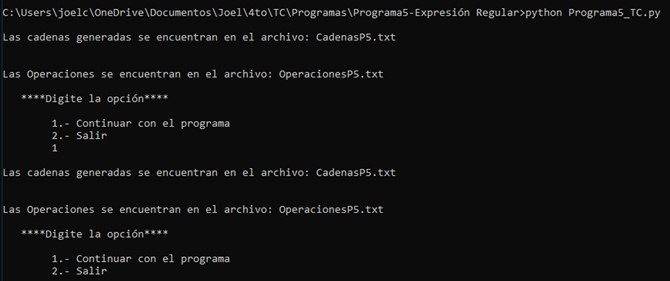
\includegraphics[height = 4cm]{main.jpg}
	
	En la imagen superior, se puede observar que se generan las primeras 10 cadenas, posterior a eso, se le vuelve a preguntar al usuario si desea que continue el programa. Para las capturas que se encuentran debajo, se considero que se generen 20 cadenas es decir que se repita 2 veces.
	\begin{enumerate}
		\item \textbf{Capturas de las Cadenas}
		\begin{itemize}
			\item 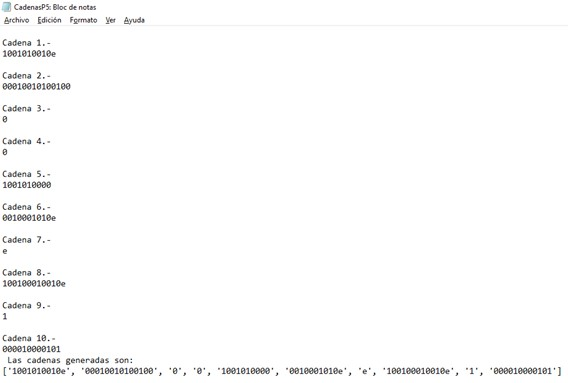
\includegraphics[height = 4cm]{Cad1.jpg}
			\item 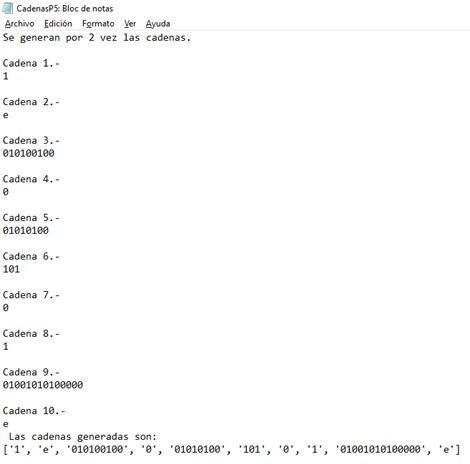
\includegraphics[height = 4cm]{Cad2.jpg}
		\end{itemize}				
		\item \textbf{Capturas de las Operaciones}
		\begin{itemize}
			\item 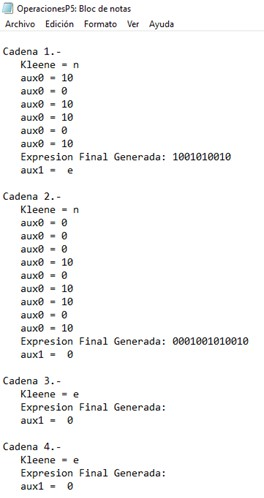
\includegraphics[height = 4cm]{Op11.jpg}
			\item 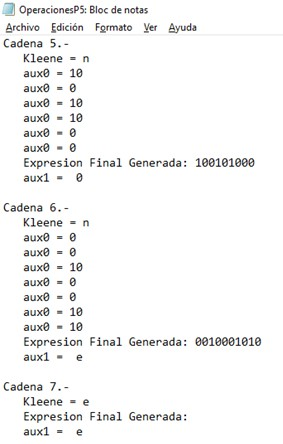
\includegraphics[height = 4cm]{Op12.jpg}
			\item 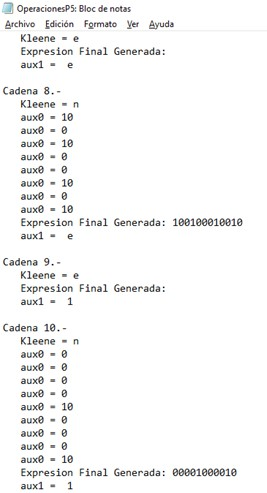
\includegraphics[height = 4cm]{Op13.jpg}
			\item 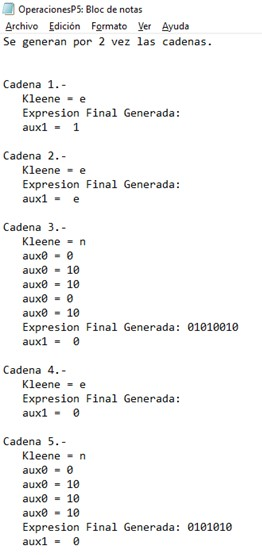
\includegraphics[height = 4cm]{Op21.jpg}
			\item 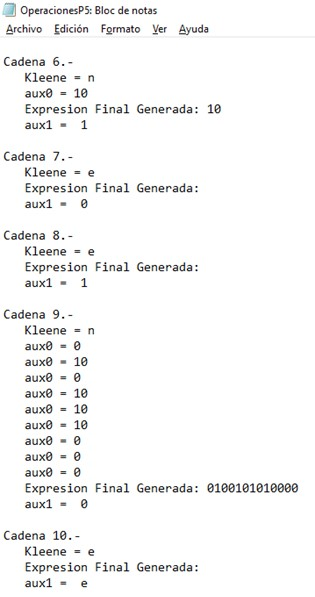
\includegraphics[height = 4cm]{Op22.jpg}
		\end{itemize}
		
		
	\end{enumerate}
	
	\section*{Código}
	\begin{python}
	# Programa 5.Expresión Regular
	# Nombre: Colín Ramiro Joel
	# Profesor: Juarez Martínez Genaro
	# Grupo: 4CM2
	# Materia: Teoría Computacional
	import random
	from tkinter import*
	def generadorCad():
		numCad = 10
		expresionGen = []    
		for i in range(0,numCad):
			archivo.write("\nCadena "+ str(i+1) + ".-")
			archivo2.write("\n\nCadena "+ str(i+1) + ".-")
			expresionGen.append ("")
			kleene = random.choice(["e","n"])
			archivo2.write("\n   Kleene = " + kleene)
			if (kleene == "n"):
				n = random.randint(1,1000)
				for j in range (0,n):
					aux0 = random.choice(["0","10"])        
					archivo2.write("\n   aux0 = " + aux0)
					expresionGen[i] = expresionGen[i] + aux0
			archivo2.write("\n   Expresion Final Generada: " + expresionGen[i])
			aux1 = random.choice(["e","0","1"])
			expresionGen[i] = expresionGen [i] + aux1
			archivo2.write(" " + "\n   aux1 =  " + aux1 )
			archivo.write("\n"+ expresionGen[i]+ "\n ")
		archivo.write("Las cadenas generadas son:\n"+ str(expresionGen))
		print("\nLas cadenas generadas se encuentran en el archivo: CadenasP5.txt\n")
		print("\nLas Operaciones se encuentran en el archivo: OperacionesP5.txt\n")
	
	opc = 1
	salir = 2
	archivo = open("CadenasP5.txt","w")
	archivo2 = open("OperacionesP5.txt","w")
	cont = 1
	while opc != salir:
		generadorCad()  			
		while (opc != salir): 
			print("   ****Digite la opción****")
			opc = int(input('''
			1.- Continuar con el programa
			2.- Salir
			'''))
			if (opc == 1):
				cont = cont + 1
				archivo.write("\n\nSe generan por " + str(cont) + " vez las cadenas.\n")
				archivo2.write("\n\nSe generan por " + str(cont) + " vez las cadenas.\n")
				generadorCad()  
			elif opc == 2:
				print("Saliendo del Programa. Hasta Luego!!!!")         
			else:
				print("Opcion inválida, Vuelva a intentar")
	\end{python}
	
	\section*{Conclusiones}
	Al término de la realización y codificación de este programa pude reforzar y más que nada terminar de entender este tema tan amplio como lo son las expresiones regulares. Me apoye de los conocimientos adquiridos en clase, asi como
 	de las láminas del curso de \textbf{Stanford}.
 	 	
 	Considero que fue un poco complicado el entendimiento total del tema y puedo decir que este fue de los programas más complejos si consideramos el tiempo efectivo tanto de codificación como de entendimiento. 	
 	No obstante ha sido  un programa el cual me apoyó para aprender y reforzar conocimientos del lenguaje de programación \textbf{Python.}
	\section*{Referencias}
	\begin{enumerate}
		\item Software Guru. (2014). Expresiones Regulares.. Diciembre 21, 2021, de Software Guru Sitio web: https://sg.com.mx/content/view/545
		\item Google. (2019). Acerca de las expresiones regulares (regex). Diciembre 21, 2021, de Google Sitio web: https://support.google.com/analytics/answer/1034324?hl=es
		\item IBM Corporation. (2015). Expresiones regulares. Diciembre 21, 2021, de IBM Corporation Sitio web: https://www.ibm.com/docs/es/i/7.3?topic=expressions-regular
		
	\end{enumerate}
\end{document}